\hypertarget{libthinkpad_8c}{
\section{libthinkpad.c File Reference}
\label{libthinkpad_8c}\index{libthinkpad.c@{libthinkpad.c}}
}


{\tt \#include $<$stdio.h$>$}\par
{\tt \#include $<$errno.h$>$}\par
{\tt \#include $<$wait.h$>$}\par
{\tt \#include $<$unistd.h$>$}\par
{\tt \#include \char`\"{}libthinkpad.h\char`\"{}}\par


Include dependency graph for libthinkpad.c:\nopagebreak
\begin{figure}[H]
\begin{center}
\leavevmode
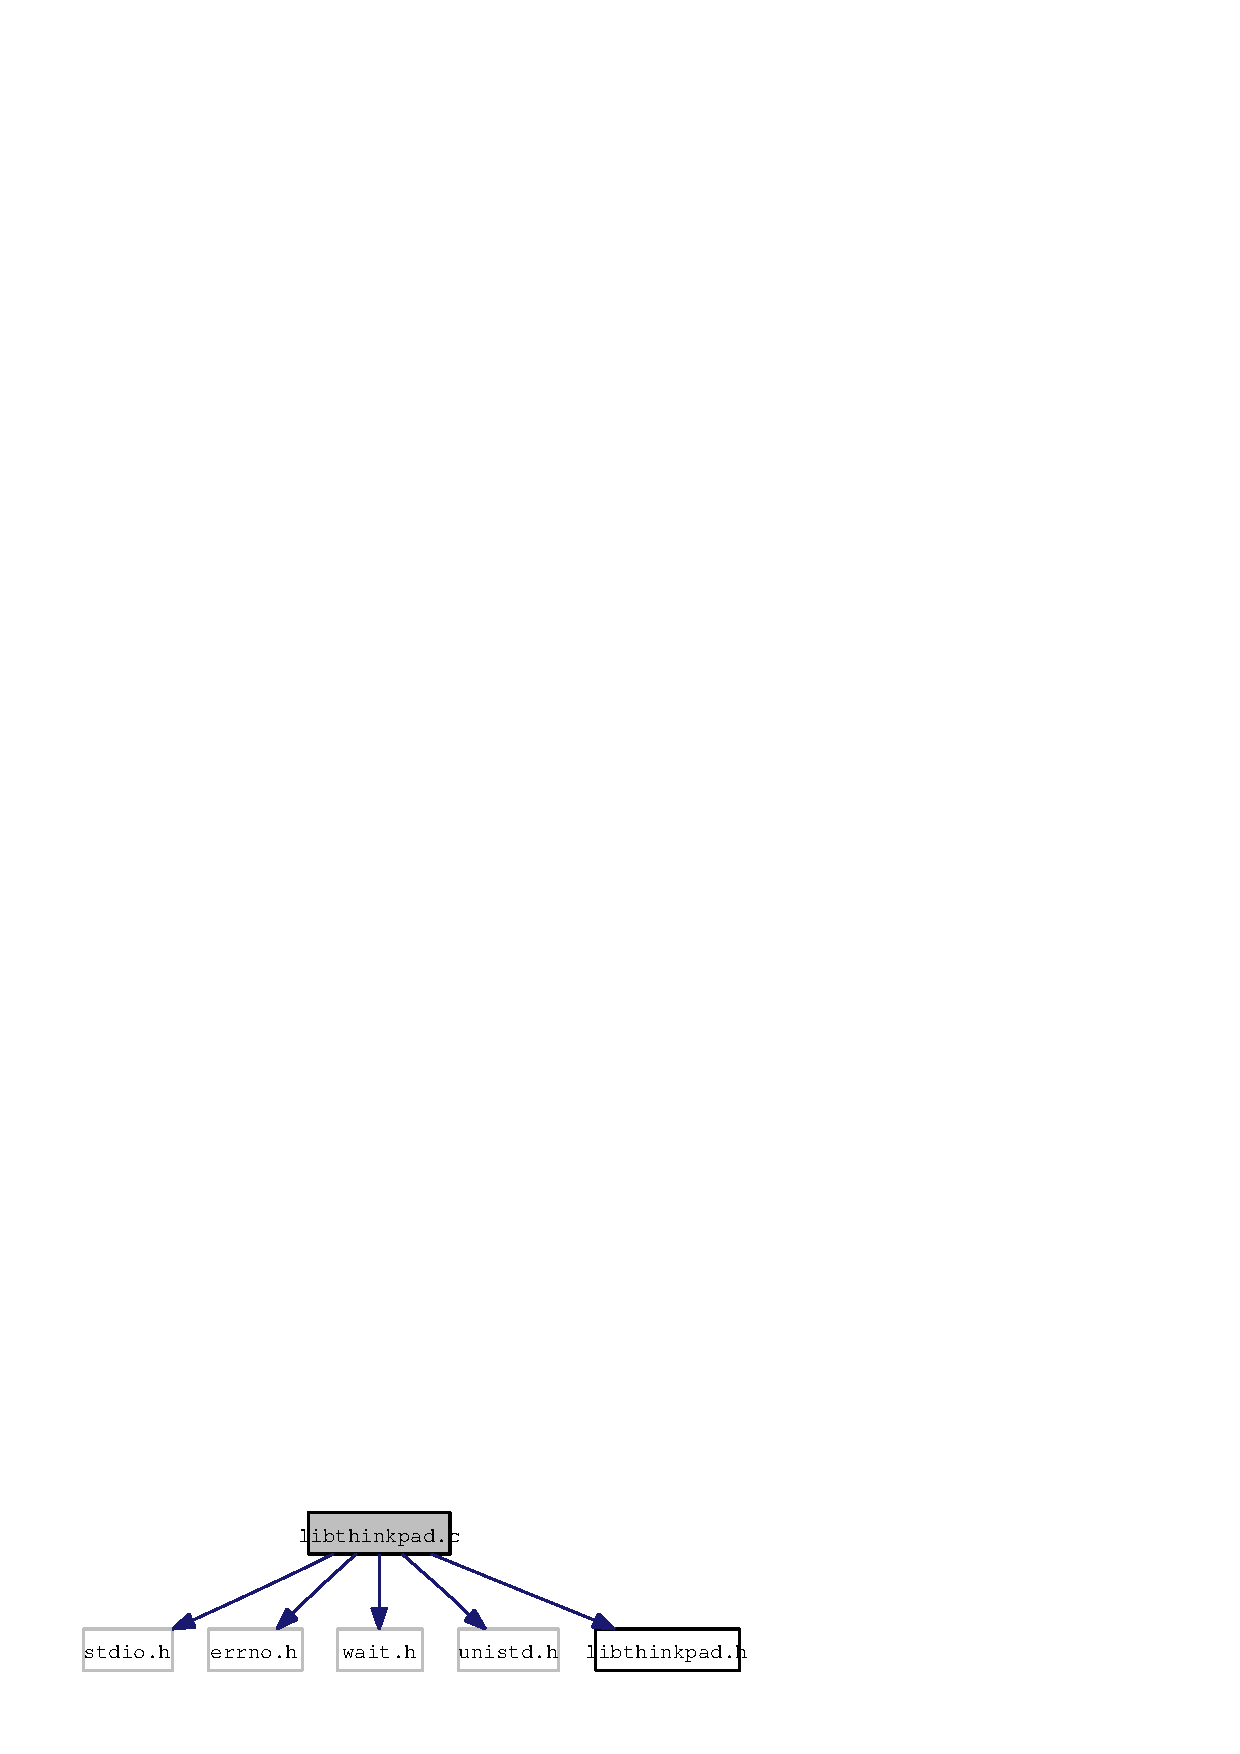
\includegraphics[width=179pt]{libthinkpad_8c__incl}
\end{center}
\end{figure}
\subsection*{Data Structures}
\begin{CompactItemize}
\item 
struct \hyperlink{structMorsecode}{Morsecode}
\end{CompactItemize}
\subsection*{Defines}
\begin{CompactItemize}
\item 
\#define \hyperlink{libthinkpad_8c_6eb92460cacc8cb18d42685f52181dd7}{MORSPOINT}~blinkLight(morse $\rightarrow$ point, 0, 1);
\item 
\#define \hyperlink{libthinkpad_8c_8c6f75e72798d81943388b4ef96fb7dd}{MORSLINE}~blinkLight(morse $\rightarrow$ line, 0, 1);
\end{CompactItemize}
\subsection*{Functions}
\begin{CompactItemize}
\item 
int \hyperlink{libthinkpad_8c_90f318656de4ddfd918141e20059474b}{blinkLight} (int on, int off, int num)
\item 
int \hyperlink{libthinkpad_8c_1c8a5a0db5fb813f149d4145c7d4a475}{blinkMorseChar} (char c)
\item 
int \hyperlink{libthinkpad_8c_b6b786c548e54b5dfc7697591c9211a6}{blinkMorseString} (char c\mbox{[}$\,$\mbox{]})
\end{CompactItemize}
\subsection*{Variables}
\begin{CompactItemize}
\item 
struct \hyperlink{structMorsecode}{Morsecode} \hyperlink{libthinkpad_8c_924cc52c5074766a5fa2ecce3c609d84}{morsecode}
\end{CompactItemize}


\subsection{Define Documentation}
\hypertarget{libthinkpad_8c_8c6f75e72798d81943388b4ef96fb7dd}{
\index{libthinkpad.c@{libthinkpad.c}!MORSLINE@{MORSLINE}}
\index{MORSLINE@{MORSLINE}!libthinkpad.c@{libthinkpad.c}}
\subsubsection{\setlength{\rightskip}{0pt plus 5cm}\#define MORSLINE~blinkLight(morse $\rightarrow$ line, 0, 1);}}
\label{libthinkpad_8c_8c6f75e72798d81943388b4ef96fb7dd}




Definition at line 37 of file libthinkpad.c.

Referenced by blinkMorseChar().\hypertarget{libthinkpad_8c_6eb92460cacc8cb18d42685f52181dd7}{
\index{libthinkpad.c@{libthinkpad.c}!MORSPOINT@{MORSPOINT}}
\index{MORSPOINT@{MORSPOINT}!libthinkpad.c@{libthinkpad.c}}
\subsubsection{\setlength{\rightskip}{0pt plus 5cm}\#define MORSPOINT~blinkLight(morse $\rightarrow$ point, 0, 1);}}
\label{libthinkpad_8c_6eb92460cacc8cb18d42685f52181dd7}




Definition at line 36 of file libthinkpad.c.

Referenced by blinkMorseChar().

\subsection{Function Documentation}
\hypertarget{libthinkpad_8c_90f318656de4ddfd918141e20059474b}{
\index{libthinkpad.c@{libthinkpad.c}!blinkLight@{blinkLight}}
\index{blinkLight@{blinkLight}!libthinkpad.c@{libthinkpad.c}}
\subsubsection{\setlength{\rightskip}{0pt plus 5cm}int blinkLight (int {\em on}, int {\em off}, int {\em num})}}
\label{libthinkpad_8c_90f318656de4ddfd918141e20059474b}


Switch the light over the lcd on and off (blinking).

\begin{Desc}
\item[Parameters:]
\begin{description}
\item[{\em on}]The time how long the light is switched on \item[{\em off}]The time how long the light is switched off \item[{\em num}]How often the light switching between on and off\end{description}
\end{Desc}
\begin{Desc}
\item[Returns:]The return value is 0 if all is okay or -1 if they was an error \end{Desc}


Definition at line 50 of file libthinkpad.c.

References LIGHTPROC.

Referenced by main().

Here is the caller graph for this function:\nopagebreak
\begin{figure}[H]
\begin{center}
\leavevmode
\includegraphics[width=87pt]{libthinkpad_8c_90f318656de4ddfd918141e20059474b_icgraph}
\end{center}
\end{figure}
\hypertarget{libthinkpad_8c_1c8a5a0db5fb813f149d4145c7d4a475}{
\index{libthinkpad.c@{libthinkpad.c}!blinkMorseChar@{blinkMorseChar}}
\index{blinkMorseChar@{blinkMorseChar}!libthinkpad.c@{libthinkpad.c}}
\subsubsection{\setlength{\rightskip}{0pt plus 5cm}int blinkMorseChar (char {\em c})}}
\label{libthinkpad_8c_1c8a5a0db5fb813f149d4145c7d4a475}


This function takes a char, and blinks than the letter in morsecode. \hyperlink{structMorsecode}{Morsecode} (\char`\"{}.\char`\"{} = short alias point, \char`\"{}-\char`\"{} = long alias line):

a -$>$ .- n -$>$ -. b -$>$ -... o -$>$ --- c -$>$ -.-. p -$>$ .--. d -$>$ -.. q -$>$ --.- e -$>$ . r -$>$ .-. f -$>$ ..-. s -$>$ ... g -$>$ --. t -$>$ - h -$>$ .... u -$>$ ..- i -$>$ .. v -$>$ ...- j -$>$ .--- w -$>$ .-- k -$>$ -.- x -$>$ -..- l -$>$ .-.. y -$>$ -.-- m -$>$ -- z -$>$ --..

1 -$>$ .---- 6 -$>$ -.... 2 -$>$ ..--- 7 -$>$ --... 3 -$>$ ...-- 8 -$>$ ---.. 4 -$>$ ....- 9 -$>$ ----. 5 -$>$ ..... 0 -$>$ -----

\begin{Desc}
\item[Parameters:]
\begin{description}
\item[{\em c}]The char for the morsecode\end{description}
\end{Desc}
\begin{Desc}
\item[Returns:]int The return value is 0 if all is okay or -1 if they was an error \end{Desc}


Definition at line 75 of file libthinkpad.c.

References Morsecode::line, morsecode, MORSLINE, MORSPOINT, Morsecode::pause, Morsecode::pausechar, Morsecode::pauseword, and Morsecode::point.

Referenced by blinkMorseString(), and main().

Here is the caller graph for this function:\nopagebreak
\begin{figure}[H]
\begin{center}
\leavevmode
\includegraphics[width=161pt]{libthinkpad_8c_1c8a5a0db5fb813f149d4145c7d4a475_icgraph}
\end{center}
\end{figure}
\hypertarget{libthinkpad_8c_b6b786c548e54b5dfc7697591c9211a6}{
\index{libthinkpad.c@{libthinkpad.c}!blinkMorseString@{blinkMorseString}}
\index{blinkMorseString@{blinkMorseString}!libthinkpad.c@{libthinkpad.c}}
\subsubsection{\setlength{\rightskip}{0pt plus 5cm}int blinkMorseString (char {\em c}\mbox{[}$\,$\mbox{]})}}
\label{libthinkpad_8c_b6b786c548e54b5dfc7697591c9211a6}




Definition at line 407 of file libthinkpad.c.

References blinkMorseChar(), Morsecode::line, morsecode, Morsecode::pause, Morsecode::pausechar, Morsecode::pauseword, and Morsecode::point.

Referenced by main().

Here is the call graph for this function:\nopagebreak
\begin{figure}[H]
\begin{center}
\leavevmode
\includegraphics[width=125pt]{libthinkpad_8c_b6b786c548e54b5dfc7697591c9211a6_cgraph}
\end{center}
\end{figure}


Here is the caller graph for this function:\nopagebreak
\begin{figure}[H]
\begin{center}
\leavevmode
\includegraphics[width=102pt]{libthinkpad_8c_b6b786c548e54b5dfc7697591c9211a6_icgraph}
\end{center}
\end{figure}


\subsection{Variable Documentation}
\hypertarget{libthinkpad_8c_924cc52c5074766a5fa2ecce3c609d84}{
\index{libthinkpad.c@{libthinkpad.c}!morsecode@{morsecode}}
\index{morsecode@{morsecode}!libthinkpad.c@{libthinkpad.c}}
\subsubsection{\setlength{\rightskip}{0pt plus 5cm}struct {\bf Morsecode}  {\bf morsecode}}}
\label{libthinkpad_8c_924cc52c5074766a5fa2ecce3c609d84}




Referenced by blinkMorseChar(), and blinkMorseString().